%beamer

% This video for Turing:
% https://www.youtube.com/watch?v=VxvY4rI15sM

% Comment/uncomment this line to toggle handout mode
% \newcommand{\handout}{}

%% Beamer-Klasse im korrekten Modus
\ifdefined \handout
\documentclass[handout]{beamer} % Handout mode
\else
\documentclass{beamer}
\fi

%% UTF-8-Encoding
\usepackage[utf8]{inputenc}

% % \bigtimes abgeschrieben von http://tex.stackexchange.com/questions/14386/importing-a-single-symbol-from-a-different-font
% \DeclareFontFamily{U}{mathx}{\hyphenchar\font45}
% \DeclareFontShape{U}{mathx}{m}{n}{
%       <5> <6> <7> <8> <9> <10> gen * mathx
%       <10.95> mathx10 <12> <14.4> <17.28> <20.74> <24.88> mathx12
%       }{}
% \DeclareSymbolFont{mathx}{U}{mathx}{m}{n}
% \DeclareMathSymbol{\bigtimes}{\mathop}{mathx}{161}

\RequirePackage{xcolor}

\def\9{\square}
%\def\9{\blank}

% f"ur Aussagenlogik
\colorlet{alcolor}{blue}
\RequirePackage{tikz}
\usetikzlibrary{arrows.meta}
\newcommand{\alimpl}{\mathrel{\tikz[x={(0.1ex,0ex)},y={(0ex,0.1ex)},>={Classical TikZ Rightarrow[]}]{\draw[alcolor,->,line width=0.7pt,line cap=round] (0,0) -- (15,0);\path (0,-6);}}}
\newcommand{\aleqv}{\mathrel{\tikz[x={(0.1ex,0ex)},y={(0ex,0.1ex)},>={Classical TikZ Rightarrow[]}]{\draw[alcolor,<->,line width=0.7pt,line cap=round] (0,0) -- (18,0);\path (0,-6);}}}
\newcommand{\aland}{\mathbin{\raisebox{-0.6pt}{\rotatebox{90}{\texttt{\color{alcolor}\char62}}}}}
\newcommand{\alor}{\mathbin{\raisebox{-0.8pt}{\rotatebox{90}{\texttt{\color{alcolor}\char60}}}}}
%\newcommand{\ali}[1]{_{\mathtt{\color{alcolor}#1}}}
\newcommand{\alv}[1]{\mathtt{\color{alcolor}#1}}
\newcommand{\alnot}{\mathop{\tikz[x={(0.1ex,0ex)},y={(0ex,0.1ex)}]{\draw[alcolor,line width=0.7pt,line cap=round,line join=round] (0,0) -- (10,0) -- (10,-4);\path (0,-8) ;}}}
\newcommand{\alP}{\alv{P}} %ali{#1}}
%\newcommand{\alka}{\negthinspace\hbox{\texttt{\color{alcolor}(}}}
\newcommand{\alka}{\negthinspace\text{\texttt{\color{alcolor}(}}}
%\newcommand{\alkz}{\texttt{\color{alcolor})}}\negthinspace}
\newcommand{\alkz}{\text{\texttt{\color{alcolor})}}\negthinspace}
\newcommand{\AAL}{A_{AL}}
\newcommand{\LAL}{\hbox{\textit{For}}_{AL}}
\newcommand{\AxAL}{\hbox{\textit{Ax}}_{AL}}
\newcommand{\AxEq}{\hbox{\textit{Ax}}_{Eq}}
\newcommand{\AxPL}{\hbox{\textit{Ax}}_{PL}}
\newcommand{\AALV}{\hbox{\textit{Var}}_{AL}}
\newcommand{\MP}{\hbox{\textit{MP}}}
\newcommand{\GEN}{\hbox{\textit{GEN}}}
\newcommand{\W}{\ensuremath{\hbox{\textbf{w}}}\xspace}
\newcommand{\F}{\ensuremath{\hbox{\textbf{f}}}\xspace}
\newcommand{\WF}{\ensuremath{\{\W,\F\}}\xspace}
\newcommand{\val}{\hbox{\textit{val}}}
\newcommand{\valDIb}{\val_{D,I,\beta}}

\newcommand*{\from}{\colon}

% die nachfolgenden Sachen angepasst an cmtt
\newlength{\ttquantwd}
\setlength{\ttquantwd}{1ex}
\newlength{\ttquantht}
\setlength{\ttquantht}{6.75pt}
\def\plall{%
  \tikz[line width=0.67pt,line cap=round,line join=round,baseline=(B),alcolor] {
    \draw (-0.5\ttquantwd,\ttquantht) -- node[coordinate,pos=0.4] (lll){} (-0.25pt,-0.0pt) -- (0.25pt,-0.0pt) -- node[coordinate,pos=0.6] (rrr){} (0.5\ttquantwd,\ttquantht);
    \draw (lll) -- (rrr);
    \coordinate (B) at (0,-0.35pt);
  }%
}
\def\plexist{%
  \tikz[line width=0.67pt,line cap=round,line join=round,baseline=(B),alcolor] {
    \draw (-0.9\ttquantwd,\ttquantht) -- (0,\ttquantht) -- node[coordinate,pos=0.5] (mmm){} (0,0) --  (-0.9\ttquantwd,0);
    \draw (mmm) -- ++(-0.75\ttquantwd,0);
    \coordinate (B) at (0,-0.35pt);
  }\ensuremath{\,}%
}
\let\plexists=\plexist
\newcommand{\NT}[1]{\ensuremath{\langle\mathrm{#1} \rangle}}

\newcommand{\CPL}{\text{\itshape Const}_{PL}}
\newcommand{\FPL}{\text{\itshape Fun}_{PL}}
\newcommand{\RPL}{\text{\itshape Rel}_{PL}}
\newcommand{\VPL}{\text{\itshape Var}_{PL}}
\newcommand{\ATer}{A_{\text{\itshape Ter}}}
\newcommand{\ARel}{A_{\text{\itshape Rel}}}
\newcommand{\AFor}{A_{\text{\itshape For}}}
\newcommand{\LTer}{L_{\text{\itshape Ter}}}
\newcommand{\LRel}{L_{\text{\itshape Rel}}}
\newcommand{\LFor}{L_{\text{\itshape For}}}
\newcommand{\NTer}{N_{\text{\itshape Ter}}}
\newcommand{\NRel}{N_{\text{\itshape Rel}}}
\newcommand{\NFor}{N_{\text{\itshape For}}}
\newcommand{\PTer}{P_{\text{\itshape Ter}}}
\newcommand{\PRel}{P_{\text{\itshape Rel}}}
\newcommand{\PFor}{P_{\text{\itshape For}}}

\newcommand{\plka}{\alka}
\newcommand{\plkz}{\alkz}
%\newcommand{\plka}{\plfoo{(}}
%\newcommand{\plkz}{\plfoo{)}}
\newcommand{\plcomma}{\hbox{\texttt{\color{alcolor},}}}
\newcommand{\pleq}{{\color{alcolor}\,\dot=\,}}

% MODIFIED (DJ)
% previously: \newcommand{\plfoo}[1]{\mathtt{\color{alcolor}#1}}
\newcommand{\plfoo}[1]{\texttt{\color{alcolor}#1}}

\newcommand{\plc}{\plfoo{c}}
\newcommand{\pld}{\plfoo{d}}
\newcommand{\plf}{\plfoo{f}}
\newcommand{\plg}{\plfoo{g}}
\newcommand{\plh}{\plfoo{h}}
\newcommand{\plx}{\plfoo{x}}
\newcommand{\ply}{\plfoo{y}}
\newcommand{\plz}{\plfoo{z}}
\newcommand{\plR}{\plfoo{R}}
\newcommand{\plS}{\plfoo{S}}

\newcommand{\bv}{\mathrm{bv}}
\newcommand{\fv}{\mathrm{fv}}

%\newcommand{\AxAL}{\hbox{\textit{Ax}}_{AL}}
%\newcommand{\AALV}{\hbox{\textit{Var}}_{AL}}

%\renewcommand{\#}[1]{\literal{#1}}
\newcommand{\A}{\mathcal{A}}
\newcommand{\Adr}{\text{Adr}}
\newcommand{\ar}{\mathrm{ar}}
\newcommand{\ascii}[1]{\literal{\char#1}}
%\newcommand{\assert}[1]{\text{/\!\!/\ } #1}
\newcommand{\assert}[1]{\colorbox{black!7!white}{\ensuremath{\{\;#1\;\}}}}
\newcommand{\Assert}[1]{$\langle$\textit{#1}$\rangle$}
\newcommand{\B}{\mathcal{B}}
\newcommand{\bfmod}{\mathbin{\kw{ mod }}}
\newcommand{\bb}{{\text{bb}}}
\def\bottom{\hbox{\small$\pmb{\bot}$}}
\newcommand{\card}[1]{|#1|}
%\newcommand{\cod}{\mathop{\text{cod}}}  % ist in thwmathabbrevs
\newcommand{\Conf}{\mathcal{C}}
\newcommand{\define}[1]{\emph{#1}}
%\renewcommand{\dh}{d.\,h.\@\xspace}
%\newcommand{\Dh}{D.\,h.\@\xspace}
%\newcommand{\engl}[1]{engl.\xspace\emph{#1}}
\newcommand{\eps}{\varepsilon}
%\newcommand{\evtl}{evtl.\@\xspace}
\newcommand{\fbin}{\text{bin}}
\newcommand{\finv}{\text{inv}}
\newcommand{\fnum}{\text{num}}
\newcommand{\fNum}{{\text{Num}}}
\newcommand{\frepr}{\text{repr}}
\newcommand{\fRepr}{\text{Repr}}
\newcommand{\fZkpl}{\text{Zkpl}}
\newcommand{\fLen}{\text{Len}}
\newcommand{\fsem}{\text{sem}}
\providecommand{\fspace}{\mathord{\text{space}}}
\providecommand{\fSpace}{\mathord{\text{Space}}}
\providecommand{\ftime}{\mathord{\text{time}}}
\providecommand{\fTime}{\mathord{\text{Time}}}
\newcommand{\fTrans}{\text{Trans}}
\newcommand{\fVal}{\text{Val}}

% Modified (DJ)
\newcommand{\Val}{\text{Val}}

%\def\G{\mathbb{Z}}
\newcommand{\HT}[1]{\normalfont\textsc{HT-#1}}
\newcommand{\htr}[3]{\{#1\}\;#2\; \{#3\}}
\newcommand{\Id}{\text{I}}
%\newcommand{\ie}{i.\,e.\@\xspace}
\newcommand{\instr}[2]{\texttt{#1}\ \textit{#2}}
\newcommand{\Instr}[2]{\texttt{#1}\ \textrm{#2}}
\newcommand{\instrr}[3]{\texttt{#1}\ \textit{#2}\texttt{(#3)}}
\newcommand{\Instrr}[3]{\texttt{#1}\ \textrm{#2}\texttt{(#3)}}
\newcommand{\io}{\!\mid\!}
\usepackage{KITcolors}
\newcommand{\literal}[1]{\hbox{\textcolor{blue!95!white}{\textup{\texttt{\scalebox{1.11}{#1}}}}}}
%\newcommand{\literal}[1]{\hbox{\textcolor{KITblue!80!black}{\textup{\texttt{#1}}}}}
\def\kasten#1{\leavevmode\literal{\setlength{\fboxsep}{1pt}\fbox{\vrule  width 0pt height 1.5ex depth 0.5ex #1}}}
\newcommand{\kw}[1]{\ensuremath{\mathbf{#1}}}
\newcommand{\lang}[1]{\ensuremath{\langle#1\rangle}}
%\newcommand{\maw}{m.\,a.\,w.\@\xspace}
%\newcommand{\MaW}{M.\,a.\,w.\@\xspace}
\newcommand{\mdefine}[2][FOOBAR]{\define{#2}\def\foobar{FOOBAR}\def\optarg{#1}\ifx\foobar\optarg\def\optarg{#2}\fi\graffito{\optarg}}
\newcommand{\meins}{\rotatebox[origin=c]{180}{1}}
\newcommand{\Mem}{\text{Mem}}
\newcommand{\memread}{\text{memread}}
\newcommand{\memwrite}{\text{memwrite}}
\providecommand{\meta}[1]{\ensuremath{\langle}\textit{#1}\ensuremath{\rangle}}
%\newcommand{\N}{\mathbb{N}}
\newcommand{\NP}{\mathbf{NP}}
\newcommand{\Nadd}{N_{\text{add}}}
\newcommand{\Nmult}{N_{\text{mult}}}
\newcommand{\Oh}[1]{O\left(#1\right)}
\newcommand{\Om}[1]{\Omega\left(#1\right)}
\newcommand{\personname}[1]{\textsc{#1}}
\newcommand{\regname}[1]{\texttt{#1}}
\newcommand{\mima}{\textsc{Mima}\xspace}
\newcommand{\mimax}{\textsc{Mima-X}\xspace}

\def\Pclass{\text{\bfseries P}}
\def\PSPACE{\text{\bfseries PSPACE}}

\newcommand{\SPush}{\text{push}}
\newcommand{\SPop}{\text{pop}}
\newcommand{\SPeek}{\text{peek}}
\newcommand{\STop}{\text{top}}
\newcommand{\STos}{\text{\itshape tos}}
\newcommand{\SBos}{\text{\itshape bos}}

%\newcommand{\R}{\mathbb{R}}
\newcommand{\Rnullplus}{\R_0^{+}}
\newcommand{\Rplus}{\R_{+}}
\newcommand{\resp}{resp.\@\xspace}
\newcommand{\Sem}{\text{Sem}}
\newcommand{\sgn}{\mathop{\text{sgn}}}
\newcommand{\sqbox}{\mathop{\raisebox{-6.2pt}{\hbox{\hbox to 0pt{$^{^{\sqcap}}$\hss}$^{^{\sqcup}}$}}}}
\newcommand{\sqleq}{\sqsubseteq}
\newcommand{\sqgeq}{\sqsupseteq}
\newcommand{\Th}[1]{\Theta\left(#1\right)}
%\newcommand{\usw}{usw.\@\xspace}
\newcommand{\V}[1]{\hbox{\textit{#1}}}
\newcommand{\x}{\times}
\newcommand{\ZK}{\mathbb{K}}
%\newcommand{\Z}{\mathbb{Z}}
%\newcommand{\zB}{z.\,B.\@\xspace}
%\newcommand{\ZB}{Z.\,B.\@\xspace}
% \newcommand{\bb}{{\text{bb}}}
% \def\##1{\hbox{\textcolor{darkblue}{\texttt{#1}}}}
% \def\A{\mathcal{A}}
% \newcommand{\0}{\#0}
% \newcommand{\1}{\#1}
% \newcommand{\Obj}{\text{Obj}}
% \newcommand{\start}{\mathop{\text{start}}}
% \newcommand{\compactlist}{\addtolength{\itemsep}{-\parskip}}
% \newcommand{\fval}{\text{val}}
% \newcommand{\lang}[1]{\ensuremath{\langle#1\rangle}}
% \newcommand{\io}{\!\mid\!}
% \def\sqbox{\mathop{\raisebox{-6.2pt}{\hbox{\hbox to 0pt{$^{^{\sqcap}}$\hss}$^{^{\sqcup}}$}}}}
% \def\sqleq{\sqsubseteq}
% \def\sqgeq{\sqsupseteq}
\def\Td{T_{\overline{d}}}
% \newcommand{\csym}[1]{\ensuremath{\#{c}_{\#{\hbox{\scriptsize #1}}}}}
% \newcommand{\F}{\ensuremath{\mathcal{F}}}
% \newcommand{\fsym}[2]{\ensuremath{\#{f}^{\#{\hbox{\scriptsize #1}}}_{\#{\hbox{\scriptsize #2}}}}}
% \newcommand{\rsym}[2]{\ensuremath{\#{R}^{\#{\hbox{\scriptsize #1}}}_{\#{\hbox{\scriptsize #2}}}}}
% \newcommand{\xsym}[1]{\ensuremath{\#{x}_{\#{\hbox{\scriptsize #1}}}}}
% \newcommand{\I}{\mathcal{I}}
% ********************************************************************

\usepackage{../TutTexbib/thwregex}
\usepackage{environ}
\usepackage{bm}
\usepackage{calc}
\usepackage{varwidth}
\usepackage{wasysym}
\usepackage{mathtools}

%% Tabellen
\usepackage{array}
\usepackage{multicol}

%% Bibliotheken für viele mathematische Symbole
\usepackage{amsmath, amsfonts, amssymb}



% This is a configuration file with personal tutor information.
% It is therefore excluded from the git repository, so changes in this file will not conflict in git commits.

% Copy this template, rename to config.tex and add your information below.

\newcommand{\myname}{Lukas Morawietz}
\newcommand{\mymail}{lukas.morawietz@gmail.com} % Consider using your named student mail address to keep your u**** account private.
\newcommand{\mytutnumber}{31}

% Don't forget to update ILIAS url. WARNING: Underscores '_' and Ampersands '&' have to be escaped with backslashes '\'. Blame TeX, not me.
\newcommand{\myILIASurl}{https://ilias.studium.kit.edu/ilias.php?ref\_id=855240\&cmdClass=ilrepositorygui\&cmdNode=5r\&baseClass=ilrepositorygui}

% Uncommenting this will print Socrative info with here defined roomname whenever \Socrative is called.
% (Otherwise, \Socrative will remain silent.)
% \newcommand{\mysocrativeroom}{???}

%\def\ThassesTut{}
\def\DanielsTut{}

\newcommand{\aboutMeFrame}{
	\begin{frame}{Über mich}
		\myname \\
		Informatik, 9. Fachsemester (Bachelor)
		% Lebensgeschichte...
		% Stammbaum...
		% Aufarbeitung der eigenen Todesser-Vergangenheit...
	\end{frame}
}

\def\thisyear{2019}

% Update date of exam
\def\myKlausurtermin{18.~März~2020, 14:00–16:00~Uhr}

\def\mydate#1{
		  \ifnum#1=1\relax	  23. Oktober \thisyear \
	\else \ifnum#1=2\relax	  30. Oktober \thisyear \
	\else \ifnum#1=3\relax    06. November \thisyear \
	\else \ifnum#1=4\relax    13. November \thisyear \
	\else \ifnum#1=5\relax    20. November \thisyear \
	\else \ifnum#1=6\relax    27. November \thisyear \
	\else \ifnum#1=7\relax    04. Dezember \thisyear \
	\else \ifnum#1=8\relax    11. Dezember \thisyear \
	\else \ifnum#1=9\relax    18. Dezember \thisyear \
	\else \ifnum#1=10\relax   08. Januar \nextyear \
	\else \ifnum#1=11\relax   15. Januar \nextyear \
	\else \ifnum#1=12\relax   22. Januar \nextyear \
	\else \ifnum#1=13\relax   29. Januar \nextyear \
	\else \ifnum#1=14\relax   05. Februar \nextyear \
	\else \textbf{Datum undefiniert!} 
	\fi\fi\fi\fi\fi\fi\fi\fi\fi\fi\fi\fi\fi\fi
}

\def\mylasttimestext{Was letztes Mal geschah...}

\colorlet{beamerlightred}{red!40}
\colorlet{beamerlightgreen}{green!50}
\colorlet{beamerlightyellow}{yellow!50}
\colorlet{lightred}{red!30}
\colorlet{lightgreen}{green!40}
\colorlet{lightyellow}{yellow!50}
\colorlet{fullred}{red!60}
\colorlet{fullgreen}{green}

\definecolor{myalertcolor}{rgb}{1,0.33,0.24}
\setbeamercolor{alerted text}{fg=myalertcolor}

% Flag to toggle display of KIT Logo.
% If you want to conform to the official logo guidelines, 
% you are not allowed to use the logo and should disable it
% using the following flag. Just saying.
% (But it's too beautiful, so best leave this commented. :P)
%\newcommand{\noKITLogo}{}

% Toggle handout mode by including the following line before including PraeambelTut
% and removing the % at the start (but do NOT remove the % char here, otherwise handout mode will always be on!)
% Please keep handout mode off in all commits!

% \newcommand{\handout}{}



% define custom \handout command flag if handout mode is toggled  #DirtyAsHellButWell...
\only<beamer:0>{\def\handout{}} %beamer:0 == handout mode

\newcommand{\R}{\mathbb{R}}
\newcommand{\N}{\mathbb{N}}
\newcommand{\Z}{\mathbb{Z}}
\newcommand{\Q}{\mathbb{Q}}
\newcommand{\BB}{\mathbb{B}}
\newcommand{\C}{\mathbb{C}}
\newcommand{\K}{\mathbb{K}}
\newcommand{\G}{\mathbb{G}}
\newcommand{\nullel}{\mathcal{O}}
\newcommand{\einsel}{\mathds{1}}
\newcommand{\Pot}{\mathcal{P}}
\renewcommand{\O}{\text{O}}

\def\word#1{\hbox{\textcolor{blue}{\texttt{#1}}}}
\let\literal\word
\def\mword#1{\hbox{\textcolor{blue}{$\mathtt{#1}$}}}  % math word
\def\sp{\scalebox{1}[.5]{\textvisiblespace}}
\def\wordsp{\word{\sp}}

%\newcommand{\literal}[1]{\textcolor{blue}{\texttt{#1}}}
\newcommand{\realTilde}{\textasciitilde \ }
\newcommand{\setsize}[1]{\ensuremath{\left\lvert #1 \right\rvert}}
\let\size\setsize
\newcommand{\set}[1]{\left\{#1\right\}}
\newcommand{\tuple}[1]{\left(#1\right)}
\newcommand{\normalvar}[1]{\text{$#1$}}

% Modified by DJ
\let\oldemptyset\emptyset
\let\emptyset\varnothing % proper emptyset

%\definecolor{myRed}{RGB}{255,75,20}
%\colorlet{myGreen}{KITpalegreen}

%\newcounter{tfqtempcount}
%\newcommand{\truefalseQ}[4]{
%	\setcounter{tfqtempcount}{#1}
%	\addtocounter{tfqtempcount}{1}
%	\truefalseQuestion{#1}{\value{tfqtempcount}}{#2}{#3}{#4}
%}

%\newcommand{\truefalseQuestion}[5]{\item<#1-|handout:#1-> \color<#2-|handout:#2->{#3} #4 \qquad \visible<#2-|handout:#2->{#5}}

\newcommand{\boder}{\ensuremath{\mathbin{\textcolor{blue}{\vee}}}\xspace}
\newcommand{\bund}{\ensuremath{\mathbin{\textcolor{blue}{\wedge}}}\xspace}
\newcommand{\bimp}{\ensuremath{\mathrel{\textcolor{blue}{\to}}}\xspace}
\newcommand{\bgdw}{\ensuremath{\mathrel{\textcolor{blue}{\leftrightarrow}}}\xspace}
\newcommand{\bnot}{\ensuremath{\textcolor{blue}{\neg}}\xspace}
\newcommand{\bone}{\ensuremath{\textcolor{blue}{1}}\text{}}
\newcommand{\bzero}{\ensuremath{\textcolor{blue}{0}}\text{}}
\newcommand{\bleftBr}{\ensuremath{\textcolor{blue}{\texttt{(}}}\text{}}
\newcommand{\brightBr}{\ensuremath{\textcolor{blue}{\texttt{)}}}\text{}}

\newcommand{\plB}{\plfoo{B}}
\newcommand{\plE}{\plfoo{E}}

\newcommand{\summe}[2]{\sum\limits_{#1}^{#2}}
\newcommand{\limes}[1]{\lim\limits_{#1}}

%\newcommand{\numpp}{\advance \value{weeknum} by -2 \theweeknum \advance \value{weeknum} by 2}
%\newcommand{\nump}{\advance \value{weeknum} by -1 \theweeknum \advance \value{weeknum} by 1}

\newcommand{\mycomment}[1]{}
\newcommand{\Comment}[1]{}

%% DISCLAIMER START 
% It is INSANELY IMPORTANT NOT TO DO THIS OUTSIDE BEAMER CLASS! IN ARTCILE DOCUMENTS, THIS IS VERY LIKELY TO BUG AROUND!
\makeatletter%
\@ifclassloaded{beamer}%
{
	% TODO 
	% no time...
	% redefine section to ignore multiple \section calls with the same title
}%
{
	\errmessage{ERROR: section command redefinition outside of beamer class document! Please contact the author of this code.}
}%
\makeatother%
%% DISCLAIMER END

\newcounter{abc}
\newenvironment{alist}{
  \begin{list}{(\alph{abc})}{
      \usecounter{abc}\setlength{\leftmargin}{8mm}\setlength{\labelsep}{2mm}
    }
}{\end{list}}


\newcommand{\stdarraystretch}{1.20}
\renewcommand{\arraystretch}{\stdarraystretch}  % for proper row spacing in tables

\newcommand{\morescalingdelimiters}{   % for proper \left( \right) typography
	\delimitershortfall=-1pt  
	\delimiterfactor=1
}

\newcommand{\centered}[1]{\vspace{-\baselineskip}\begin{center}#1\end{center}\vspace{-\baselineskip}}

% for \implitem and \item[bla] stuff to look right:
\setbeamercolor*{itemize item}{fg=black}
\setbeamercolor*{itemize subitem}{fg=black}
\setbeamercolor*{itemize subsubitem}{fg=black}

\setbeamercolor*{description item}{fg=black}
\setbeamercolor*{description subitem}{fg=black}
\setbeamercolor*{description subsubitem}{fg=black}

\renewcommand{\qedsymbol}{\textcolor{black}{\openbox}}

\renewcommand{\mod}{\mathop{\textbf{mod}}}
\renewcommand{\div}{\mathop{\textbf{div}}}

\newcommand{\ceil}[1]{\left\lceil#1\right\rceil}
\newcommand{\floor}[1]{\left\lfloor#1\right\rfloor}
\newcommand{\abs}[1]{\left\lvert #1 \right\rvert}
\newcommand{\Matrix}[1]{\begin{pmatrix} #1 \end{pmatrix}}
\newcommand{\braced}[1]{\left\lbrace #1 \right\rbrace}

\def\fract#1/#2 {\frac{#1}{#2}} % ! Trailing space is crucial!
\def\dfract#1/#2 {\dfrac{#1}{#2}} % ! Trailing space is crucial!

\newcommand{\Mid}{\;\middle|\;}

\let\after\circ

\def\·{\cdot}
\def\*{\cdot}
\def\?>{\ensuremath{\rightsquigarrow}}  % Fuck you, Latex

\newcommand{\tight}[1]{{\renewcommand{\arraystretch}{0.76} #1}}
\newcommand{\stackedtight}[1]{{\renewcommand{\arraystretch}{0.76} \begin{matrix} #1 \end{matrix}} }
\newcommand{\stacked}[1]{\begin{matrix} #1 \end{matrix} }
\newcommand{\casesl}[1]{\delimitershortfall=0pt  \left\lbrace\hspace{-.3\baselineskip}\begin{array}{ll} #1 \end{array}\right.}
\newcommand{\casesr}[1]{\delimitershortfall=0pt  \left.\begin{array}{ll} #1 \end{array}\hspace{-.3\baselineskip}\right\rbrace}
\newcommand{\caseslr}[1]{\delimitershortfall=0pt  \left\lbrace\hspace{-.3\baselineskip}\begin{array}{ll} #1 \end{array}\hspace{-.3\baselineskip}\right\rbrace}

\def\q#1uad{\ifnum#1=0\relax\else\quad\q{\the\numexpr#1-1\relax}uad\fi}
% e.g. \q1uad = \quad, \q2uad = \qquad etc.

\newcommand{\qqquad}{\q3uad}

\newcommand{\impl}{\ifmmode\ensuremath{\mskip\thinmuskip\Rightarrow\mskip\thinmuskip}\else$\Rightarrow$\fi\xspace}
\newcommand{\Impl}{\ifmmode\implies\else$\Longrightarrow$\fi\xspace}

\newcommand{\derives}{\Rightarrow}

\newcommand{\gdw}{\ifmmode\mskip\thickmuskip\Leftrightarrow\mskip\thickmuskip\else$\Leftrightarrow$\fi\xspace}
\newcommand{\Gdw}{\ifmmode\iff\else$\Longleftrightarrow$\fi\xspace}

\newcommand{\symbitemnegoffset}{\hspace{-.5\baselineskip}}
\newcommand{\implitem}{\item[\impl\symbitemnegoffset]}
\newcommand{\Implitem}{\item[\Impl\symbitemnegoffset]}


\newcommand{\forcenewline}{\mbox{}\\}


% proper math typography
\newcommand{\functionto}{\longrightarrow}
\renewcommand{\geq}{\geqslant}
\renewcommand{\leq}{\leqslant}
\let\oldsubset\subset
\renewcommand{\subset}{\subseteq} % for all idiots out there using subset

\newenvironment{threealign}{%
	\[
	\begin{array}{r@{\ }c@{\ }l}
}{%
	\end{array}	
	\]
}

\newcommand{\concludes}{ \\ \hline  }
\newcommand{\deduction}[1]{
	\begin{varwidth}{.8\linewidth}
		\begin{tabular}{>{$}c<{$}}
			#1
		\end{tabular}
	\end{varwidth}	
}

\definecolor{hoareorange}{rgb}{1,.85,.6}
\newcommand{\hoareassert}[1]{\setlength{\fboxsep}{1pt}\setlength{\fboxrule}{-1.4pt}\fcolorbox{white}{hoareorange}{\ensuremath{\{\;#1\;\}}}\setlength\fboxrule{\defaultfboxrule}\setlength{\fboxsep}{3pt}}

\newcommand{\mailto}[1]{\href{mailto:#1}{{\textcolor{blue}{\underline{#1}}}}}
\newcommand{\urlnamed}[2]{\href{#2}{\textcolor{blue}{\underline{#1}}}}
\renewcommand{\url}[1]{\urlnamed{#1}{#1}}

\newcommand{\hanging}{\hangindent=0.7cm}
\newcommand{\indented}{\hanging}

%requires \thisyear to be defined (s. config.tex)!
\edef\nextyear{\the\numexpr\thisyear+1\relax}


% --- \frameheight constant ---
\newlength\fullframeheight
\newlength\framewithtitleheight
\setlength\fullframeheight{.92\textheight}
\setlength\framewithtitleheight{.86\textheight}

\newlength\frameheight
\setlength\frameheight{\fullframeheight}

\let\frametitleentry\relax
\let\oldframetitle\frametitle
\def\newframetitle#1{\global\def\frametitleentry{#1}\if\relax\frametitleentry\relax\else\setlength\frameheight{\framewithtitleheight}\fi\oldframetitle{#1}}
\let\frametitle\newframetitle

\def\newframetitleoff{\let\frametitle\oldframetitle}
\def\newframetitleon{\let\frametitle\newframetitle}
% --- \frameheight constant end ---



\newenvironment{headframe}{\Huge THIS IS AN ERROR. PLEASE CONTACT THE ADMIN OF THIS TEX CODE. (headframe env def failed)}{}
\RenewEnviron{headframe}[1][]{
	\begin{frame}\frametitle{\ }
		\centering
		\Huge\textbf{\textsc{\BODY} \\
		}
		\Large {#1}
		\frametitle{\ }
	\end{frame}
}


\makeatletter
% Provides color if undefined.
\newcommand{\colorprovide}[2]{%
	\@ifundefinedcolor{#1}{\colorlet{#1}{#2}}{}}
\makeatother


\colorprovide{lightred}{red!30}
\colorprovide{lightgreen}{green!40}
\colorprovide{lightyellow}{yellow!50}
\colorprovide{beamerlightred}{lightred}
\colorprovide{beamerlightgreen}{lightgreen}
\colorprovide{beamerlightyellow}{lightyellow}
\colorprovide{fullred}{red!60}
\colorprovide{fullgreen}{green}
\definecolor{darkred}{RGB}{115,48,38}
\definecolor{darkgreen}{RGB}{48,115,38}
\definecolor{darkyellow}{RGB}{100,100,0}

\only<handout:0>{\colorlet{adaptinglightred}{beamerlightred}}
\only<handout:0>{\colorlet{adaptinglightgreen}{beamerlightgreen}}
\only<handout:0>{\colorlet{adaptinglightred}{beamerlightred}}
\only<beamer:0>{\colorlet{adaptinglightred}{lightred}}
\only<beamer:0>{\colorlet{adaptinglightgreen}{lightgreen}}
\only<beamer:0>{\colorlet{adaptinglightred}{lightred}}
\only<handout:0>{\colorlet{adaptingred}{lightred}}
\only<beamer:0>{\colorlet{adaptingred}{fullred}}
\only<handout:0>{\colorlet{adaptinggreen}{lightgreen}}
\only<beamer:0>{\colorlet{adaptinggreen}{fullgreen}}



\newcommand{\TrueQuestion}[1]{
	\TrueQuestionE{#1}{}
}

\newcommand{\YesQuestion}[1]{
	\YesQuestionE{#1}{}
}

\newcommand{\FalseQuestion}[1]{
	\FalseQuestionE{#1}{}
}

\newcommand{\NoQuestion}[1]{
	\NoQuestionE{#1}{}
}

\newcommand{\DependsQuestion}[1]{
	\DependsQuestionE{#1}{}
}

\newcommand{\QuestionVspace}{\vspace{4pt}}
\newcommand{\QuestionParbox}[1]{\begin{varwidth}{.85\linewidth}#1\end{varwidth}}
\newcommand{\ExplanationParbox}[1]{\begin{varwidth}{.97\linewidth}#1\end{varwidth}}
\colorlet{questionlightgray}{gray!23}
\let\defaultfboxrule\fboxrule

% #1: bg color
% #2: fg color short answer
% #3: short answer text
% #4: question
% #5: explanation
\newcommand{\GenericQuestion}[5]{
	\setlength\fboxrule{2pt}
	\only<+|handout:0>{\hspace{-2pt}\fcolorbox{white}{questionlightgray}{\QuestionParbox{#4} \quad\textbf{?}}}
	\visible<+->{\hspace{-2pt}\fcolorbox{white}{#1}{\QuestionParbox{#4} \quad\textbf{\textcolor{#2}{#3}}} \ExplanationParbox{#5}} \\
	\setlength\fboxrule{\defaultfboxrule}
}

% #1: Q text
% #2: Explanation
\newcommand{\TrueQuestionE}[2]{
	\GenericQuestion{adaptinglightgreen}{darkgreen}{Wahr.}{#1}{#2}
}

% #1: Q text
% #2: Explanation
\newcommand{\YesQuestionE}[2]{
	\GenericQuestion{adaptinglightgreen}{darkgreen}{Ja.}{#1}{#2}
}

% #1: Q text
% #2: Explanation
\newcommand{\FalseQuestionE}[2]{
	\GenericQuestion{adaptinglightred}{darkred}{Falsch.}{#1}{#2}
}

% #1: Q text
% #2: Explanation
\newcommand{\NoQuestionE}[2]{
	\GenericQuestion{adaptinglightred}{darkred}{Nein.}{#1}{#2}
}

% #1: Q text
% #2: Explanation
\newcommand{\DependsQuestionE}[2]{
	\GenericQuestion{adaptinglightyellow}{darkyellow}{Je nachdem!}{#1}{#2}
}

\ifnum\thisyear=2017 \else \errmessage{Old ILIAS link inside preamble. Please update.} \fi

\newcommand{\ILIAS}{\urlnamed{ILIAS}{https://ilias.studium.kit.edu/ilias.php?ref\_id=729057\&cmdClass=ilrepositorygui\&cmdNode=75\&baseClass=ilrepositorygui}\xspace}

\newcommand{\Socrative}{\only<handout:0>{socrative.com $\qquad \?> $ Student login \\ Raumname:  \mysocrativeroom\\ \medskip}}

\newcommand{\thasse}[1]{
	\ifdefined\ThassesTut #1\xspace \else\fi
}
\newcommand{\daniel}[1]{
	\ifdefined\DanielsTut #1\xspace \else\fi
}
\newcommand{\thassedaniel}[2]{\ifdefined\ThassesTut #1\else\ifdefined\DanielsTut #2\fi\fi\xspace}

\ifdefined\ThassesTut \ifdefined\DanielsTut \errmessage{ERROR: Both ThassesTut and DanielsTut flags are set. This is most likely an error. Please check your config.tex file.} \else \fi \else \ifdefined\DanielsTut \else \errmessage{ERROR: Neither ThassesTut  nor DanielsTut flags are set. This is most likely an error. Please check your config.tex file.} \fi\fi

%\newcommand{\sgn}{\text{sgn}}


% Das ist der KIT-Stil
%\usepackage{../TutTexbib/beamerthemekit}
\usepackage[deutsch,titlepage0]{../TutTexbib/KIT/beamerthemeKITmod}
\TitleImage[width=\titleimagewd]{../figures/titlepage.jpg}
%\usetheme[deutsch,titlepage0]{KIT}

% Include PDFs
\usepackage{pdfpages}

% Libertine font (Original GBI font)
\usepackage{libertine}
%\renewcommand*\familydefault{\sfdefault}  %% Only if the base font of the document is to be sans serif

% Nicer math symbols
\usepackage{eulervm}
%\usepackage{mathpazo}
\renewcommand\ttdefault{cmtt} % Computer Modern typewriter font, see lecture slides.

%% Deutsche Silbentrennung und Beschriftungen
\usepackage[ngerman]{babel}



\usepackage{csquotes}



%% Anzeigetiefe für Inhaltsverzeichnis: 1 Stufe
\setcounter{tocdepth}{1}

%% Schönere Schriften
\usepackage[TS1,T1]{fontenc}

%% Bibliothek für Graphiken
\usepackage{graphicx}

%% der wird sowieso in jeder Datei gesetzt
%%\graphicspath{{../figures/}}

%% Hyperlinks
\usepackage{hyperref}
% I don't know why, but this works and only includes sections and NOT subsections in the pdf-bookmarks.
\hypersetup{bookmarksdepth=subsection} 

%\usepackage{lmodern}
\usepackage{colortbl}
\usepackage[absolute,overlay]{textpos}
\usepackage{listings}
\usepackage{forloop}
%\usepackage{algorithmic} % PseudoCode package 

\usepackage{tikz}
\usetikzlibrary{matrix}
\usetikzlibrary{arrows.meta}
\usetikzlibrary{automata}
\usetikzlibrary{tikzmark}

% Needed for gbi-macros
\usepackage{xspace}

%%%%%%%%%%%% INHALT %%%%%%%%%%%%%%%%

%% Wochennummer
\newcounter{weeknum}



%% Titelinformationen
\title[GBI-Tutorium \mytutnumber, Woche \theweeknum]{Grundbegriffe der Informatik \\ Tutorium \mytutnumber}

\subtitle{Woche \theweeknum \ | \mydate{\theweeknum} \\ \myname \ \  \normalfont (\mailto{\mymail})}
\author[\myname]{\myname}
\institute{KIT -- Karlsruher Institut für Technologie}
\date{\mydate{\theweeknum}\ }

% Modified, DJ (better safe than sorry)
\AuthorTitleSep{ – }

%% Titel einfügen
\newcommand{\titleframe}{\frame{\titlepage}}

%% Alles starten mit \starttut{X}
\newcommand{\starttut}[1]{\setcounter{weeknum}{#1}\titleframe\frame{\frametitle{Inhalt}\tableofcontents} \AtBeginSection[]{%
\begin{frame}
	\tableofcontents[currentsection]
\end{frame}\addtocounter{framenumber}{-1}}}


\newcommand{\framePrevEpisode}{
	\begin{headframe}
		\mylasttimestext
	\end{headframe}
}

%% Legacy: Lastframe. Not for further usage!
\newcommand{\lastframetitled}[5]{
	\frame[plain]{
		\vspace{-#2pt}
		\begin{figure}[H]
			\centering
			\LARGE \textbf{\textsc{#5}} \\
			\vspace{.2\baselineskip}
			\includegraphics[scale=#1]{#3}
			\vspace{-7pt}
			\caption{ \texttt{\url{#4}} }
		\end{figure} 
	}
}
\newcommand{\lastframe}[4]{\xkcdframe{#1}{#2}{#3}{#4}{}}
\newcommand{\xkcdframe}[5]{
	\frame[plain]{
		\vspace{-#2pt}
		\begin{figure}[H]
			\centering
			\includegraphics[scale=#1]{#3}
			\vspace{-7pt}
			\caption{ \texttt{\url{#4}} }
			\vspace{5pt}
			#5
		\end{figure} 
	}
}

%% Wörter
\newcommand{\code}[1]{$\mathbf{#1}$}

%% Sterne

\newcounter{starsc}
\newcommand{\stars}[1]{
	\hfill
	\begin{minipage}{100px}
		\forloop{starsc}{0}{\value{starsc} < #1}%
		{%
			
\includegraphics[scale=0.05]{star-full.pdf} \hspace*{1px}
		}%
		\forloop{starsc}{\value{starsc}}{\value{starsc} < 5}%
		{%
			
\includegraphics[scale=0.05]{star-empty.pdf} \hspace*{1px}
		}
		\vspace*{2px}
	\end{minipage}
}

% No stars for me...
\renewcommand{\stars}[1]{}

\newcommand{\slideThanks}{
	\begin{frame}
		\frametitle{Credits}
		\begin{block}{}
			Vorgänger dieses Foliensatzes wurden erstellt von:\\[1em]
			Thassilo Helmold \\
			Philipp Basler \\
			Nils Braun \\
			Dominik Doerner \\
			Ou Yue \\
		\end{block}
	\end{frame}
}

%% Verbatim
\usepackage{moreverb}
\graphicspath{{../figures/}}

\morescalingdelimiters

\begin{document}
\starttut{14}

%\thasse{\lastframe{0.55}{20}{xkcd/turing_test.png}{https://www.xkcd.com/}}

\daniel{
\begin{frame}{Zu Blatt \#6}
	Durchschnitt: \quad jeder, der regelmäßig abgab, \textbf{hat den Schein}! :D
	\begin{itemize}
		\item \textbf{A6.1}: $\fract \cdots/b $ \impl was, wenn $b = 0$? \lightning \\
		\impl Umformungen waren nicht nötig, einfach Axiome benutzen und fertig.
	\end{itemize}
\end{frame}
}

\framePrevEpisode

\begin{frame}{Rückblick: Endliche Automaten}
	\begin{itemize}[<+->]
		\item Mealy- und Moore-Automaten
		\item Formale Definition und graphische Repräsentation
		\item $f, f_*, f_{**}$
		\item $g, g_*, g_{**}$
		\item Endliche Akzeptoren
		\item Reguläre Ausdrücke
	\end{itemize}
\end{frame}

\begin{frame}[t]{Wahr oder Falsch?}
	%\Socrative
	\begin{figure}
		\begin{tikzpicture}[->,>=stealth,shorten >=1pt,auto,node distance=2cm,
		semithick,initial text={}]
		\tikzstyle{every state}=[]
		
		\node[state,accepting] (B)   {$Z_1$};
		\node[state]		 (M)  [right of=B]		{$Z_2$};
		
		\path
		(B) edge [loop above]  node {\word 1} (B) 
		(B) edge 			  node {\word 0} (M) 
		(M) edge [loop above] node {\word 0, \word 1} (M);
	\end{tikzpicture}
	\end{figure}
	
	\DependsQuestionE{Dieser Automat erkennt die Sprache $ \{\word 1\}^*$.} {Die Angabe des Startzustands fehlt. Startet man in $Z_2$, akzeptiert der Automat gar nichts.}
\end{frame}

\begin{frame}[t]{Wahr oder Falsch?}
	\FalseQuestionE{Das (komplizierte) Master-Theorem kann man immer anwenden.}{ Nur bei rekursiven Algorithmen, bei denen das Problem in gleich große Teilprobleme aufgeteilt wird.}
	\FalseQuestionE{Jeder Moore-Automat kann in einen Mealy-Automaten umgewandelt werden, der für jedes Wort die gleiche Ausgabe produziert.}{ Für das leere Wort kann ein Mealy-Automat niemals eine Ausgabe produzieren.}
	\TrueQuestionE{Endliche Akzeptoren sind Moore-Automaten mit dem Ausgabealphabet $\{\word 0,\word 1\}$.}{}
	\FalseQuestionE{Mit endlichen Automaten kann jede beliebige Sprache erkannt \\ werden.}{Tatsächlich ist die Menge der akzeptierbaren Sprachen sogar sehr eingeschränkt.}	
\end{frame}


\section{Rechtslineare Grammatiken}
\begin{frame}{Rechtslineare Grammatiken}
	\begin{Definition}
		Eine Grammatik $G = (N, T, S, P)$ nennt man \textbf{rechtslinear}, wenn bei jeder Produktion auf der rechten Seite \textbf{höchstens ein} Nichtterminalsymbol und dieses nur \textbf{als letztes} Symbol steht.\\
		D. h., alle Produktionen folgen dem Schema $$X \to w \quad \text{oder} \quad X \to wY$$ mit $w \in T^*, \; X,Y \in N$.
	\end{Definition}
\end{frame}

\begin{frame}{Reguläre Sprachen}
	\begin{Satz}
		Für jede formale Sprache $L$ sind die folgenden drei Aussagen äquivalent:
		\begin{itemize}
			\item $L$ kann von einem endlichen Akzeptor erkannt werden.
			\item $L$ kann durch einen regulären Ausdruck beschrieben werden.
			\item $L$ kann von einer rechtslinearen Grammatik erzeugt werden.
		\end{itemize}
	\end{Satz}
	
	Eine solche Sprache nennen wir \textbf{regulär}.
\end{frame}

\begin{frame}{Beispiele für Umwandlungen}
	Siehe Übung 13, WS 15/16
\end{frame}

\begin{frame}{Beispiele}
	$G = (\{X\}, \{\word a, \word b\}, X, P )$ mit 
	$$P = \set{X \to \word aX \mid \word{ba}X \mid \word b \mid \varepsilon }$$
	% Das da ist FALSCH:
	% TODO: Nein, ist es nicht. Es entspricht genau der "Umsetzung" des Automaten
	% Aber das könnte man noch besser herausarbeiten: Automat Tikzen und Zustände umbenennen, G' dann aus Automaten "ablesen"
	%$$P = \{X \to aX \mid bY \mid \varepsilon, Y \to aX \mid bZ \mid \varepsilon, Z \to aZ \mid bZ\}$$ 
	ist eine rechtslineare Grammatik. Die dadurch erzeugte Sprache ist \pause 
	$$L(G) = \set{ w \Mid \forall v_1, v_2 \in \{\word a,\word b\}^\ast: w \neq v_1 \word{bb} v_2 },$$ 
	der sie beschreibende reguläre Ausdruck ist \pause 
	$$R =  \rx{(a|ba)*(b|O*)}.  $$ 
	Der Automat dazu sieht so aus: \\ \pause
	\centering
	\begin{tikzpicture}[->,>=stealth,shorten >=1pt,auto,semithick,node distance=2cm,initial text={}]
	\tikzstyle{every state}=[]
	
	\node[initial,state,accepting] (0)                    {$0$};
	\node[state,accepting]         (1) [right of=0]       {$1$};
	\node[initial,state]           (2) [right of=1]       {$2$};
	
	\path (0) edge [loop below] node {\word a} (0);
	\path (0) edge [bend right] node [below] {\word b} (1);
	\path (1) edge [bend right] node [above] {\word a} (0);
	\path (1) edge [] node {\word b} (2);
	\path (2) edge [loop below] node {$\word a, \word b$} (2);
	\end{tikzpicture}
\end{frame}


\begin{frame}{Achtung!}
	Eine Grammatik kann nicht rechtslinear sein und \textbf{trotzdem} eine reguläre Sprache erzeugen! \\
	\bigskip
	$G = \tuple{\set{A}, \set{\word a}, A, \set{A \to \alert{AA} \mid \word a \mid \eps}}$, \quad (\alert{nicht} rechtslinear) \\ \pause
	$G' = \tuple{\set{A}, \set{\word a}, A, \set{A \to \word aA \mid \eps}}$; \quad (rechtslinear) \\ 
	\medskip
	\[\text{und } \quad L(G) = L(G') = \lang{\rx{a*}} \quad \textbf{(regulär!)}\]
\end{frame}

\begin{frame}{Noch mehr Beispiele}
	\begin{itemize}
		\item $G = (\{X \}, \{\word a,\word  b\}, X , \{X \to \word{ab}X \mid \word{bba}X \mid \varepsilon \}$, \\
			$L(G) = \lang{\visible<2-|handout:2>{\rx{(ab|bba)*}}} $
		\item $G = (\{X , Y\}, \{\word a, \word b\}, X , \{X \to \word aX \mid \word bX \mid \word{ababb}Y , Y \to \word aY \mid \word bY \mid \varepsilon \}$, \\
			$L(G) = \lang{\visible<3-|handout:2>{\rx{(a|b)*ababb(a|b)*}}} $
	\end{itemize}
\end{frame}

% Sorry, die Zeit hab ich nicht...
% Ich auch nicht, aber zum Nachlesen lasse ich es trotzdem erstmal drin.
\thasse{
	\begin{frame}{Aufgabe}
		Gegeben ist im folgenden jeweils eine Beschreibung einer formalen Sprache $L$ und ein dazugehöriges Alphabet. Schreiben Sie jeweils den regulären Ausdruck $R$ auf, für den $L(R) = L $ gilt und stellen Sie eine rechtslineare Grammatik $G$ auf, für die $L(G) = L $ gilt:
		\begin{itemize}
			\item Die Menge aller Worte über dem Alphabet $A=\{\word a,\word  b, \word c\}$, die genau ein $\word c$ enthalten. \\
			\visible<2-|handout:2>{
				\emph{Lösung}: $\rx{(a|b)*c(a|b)*}$
			}
			\item Die Menge aller Worte über dem Alphabet $A=\{\word a,\word  b\}$, bei denen die Anzahl der $\word b$ durch 3 teilbar ist. \\
			\visible<3-|handout:2>{
				\emph{Lösung}: $\rx{a*(ba*ba*ba*)*}$
			}
		\end{itemize}
	\end{frame}
	
	\begin{frame}{Aufgabe}
		\textit{Gegeben sei die rechtslineare Grammatik } $$ G= (\{S\},\{\word a,\word  b\},S,P) \qquad P = \{S\to \word{baa}S \mid \word{ba}S \mid \word{aa}S \mid \varepsilon \} $$
		\begin{itemize}
			\only<1-3|handout:1,2>{
				\item Geben Sie einen endlichen Akzeptor $A$ an, so dass $L(A) = L(G)$ gilt
				\only<3|handout:2>{
					\begin{figure}[H]
						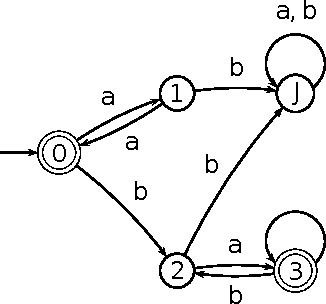
\includegraphics[scale=0.9]{regulaer/L2.pdf}
					\end{figure}
				}
			}
			\only<1,4-5|handout:1,3>{
				\item Gebt einen regulären Ausdruck $R$ an, so dass $ \lang{R} = L(G) $ gilt
				\only<5|handout:3>{
					$$ \rx{(baa|ba|aa)*}$$
				}
			}
			\only<1,6-7|handout:1,3>{
				\item Gebt einen regulären Ausdruck $R$ an, der nicht das Zeichen $\rx{|}$ enthält, und für den $\lang{R}= L(G) $ gilt.
				\only<7|handout:3>{
					$$ \rx{(aa)* (baa*)*} $$
				}
			}
		\end{itemize}
	\end{frame}
	
}



%\begin{frame}
%	\frametitle{Was wir können:}
%	Von..
%	\begin{description}
%		\item[..rechtslinearen Gammatiken..] zu
%		\begin{itemize}
%			\item den Akzeptoren: \pause (mind.) jedes Nichtterminalsymbol ein Zustand, $|$ ist Verzweigung, Akzeptierende Zustände wählen \pause
%			\item den regulären Ausdrücken: \pause Schwierig!
%		\end{itemize}
%		\item[..endlichen Akzeptoren..]  zu
%		\begin{itemize}
%			\item den Grammatiken: \pause Zustandsübergang ist eine Produktion\pause
%			\item den regulären Ausdrücken: \pause Einzelne Wege abgehen
%		\end{itemize}
%		\item[..regulären Ausdrücken..] zu
%		\begin{itemize}
%			\item den Akzeptoren: \pause in Abschnitte teilen, $\ast$ ist Schleife, $|$ ist Verzweigung \pause
%			\item den rechtslinearen Grammatiken: \pause genauso wie Akzeptor
%		\end{itemize}
%	\end{description}
%\end{frame}

\begin{frame}[t]{Wahr oder Falsch?}
	\FalseQuestionE{Jede kontextfreie Grammatik lässt sich als regulärer Ausdruck \\ darstellen.}{Die Grammatik muss dafür rechtslinear sein, kontextfrei ist \enquote{zu mächtig}.}
	\TrueQuestion{Jeder regulären Ausdruck lässt sich durch eine kontextfreie Grammatik darstellen.}
	\TrueQuestion{Für jede Sprache $L$ und jedes Wort $w \in L$ gilt: Es existiert ein endlicher Automat, der $w$ erkennt.}
	\FalseQuestion{Die Sprache der gültigen Klammerausdrücke ist regulär.}
	\TrueQuestionE{Die Sprache der gültigen Klammerausdrücke ist kontextfrei.}{}
\end{frame}

\graphicspath{{../figures/}}

\newenvironment{Messtabelle}[1]
{\begin{minipage}{\linewidth} \centering  \begin{tabular}{#1} }
{\end{tabular} \vspace*{1em} \end{minipage}} 

\section{Turingmaschinen}

\begin{frame}{Grenzen endlicher Automaten}
	Automaten haben ja keinen Speicher außer ihren Zustand. \\
	\medskip
	\impl Ändern wir das: \\
	Nehmen wir nen Mealy-Automaten und ein unendlich langes Buchstabenband, das er lesen/beschreiben kann. \\
	\medskip
	Heraus kommt die...
\end{frame}

\subsection{Inhalt}
\begin{frame}{Turingmaschine}
	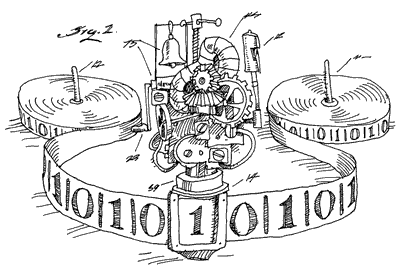
\includegraphics[scale=1]{turing/tmAufbau}
\end{frame}

% Kann ich erst Werbung für machen, nachdem ich ihn selbst gesehen habe, sonst wird's unglaubwürdig... :P
% Dann solltest du ihn unbedingt mal anschauen!
\thasse{
	\begin{frame}{Alan Turing}
		\centering
		\vspace{-25pt}
		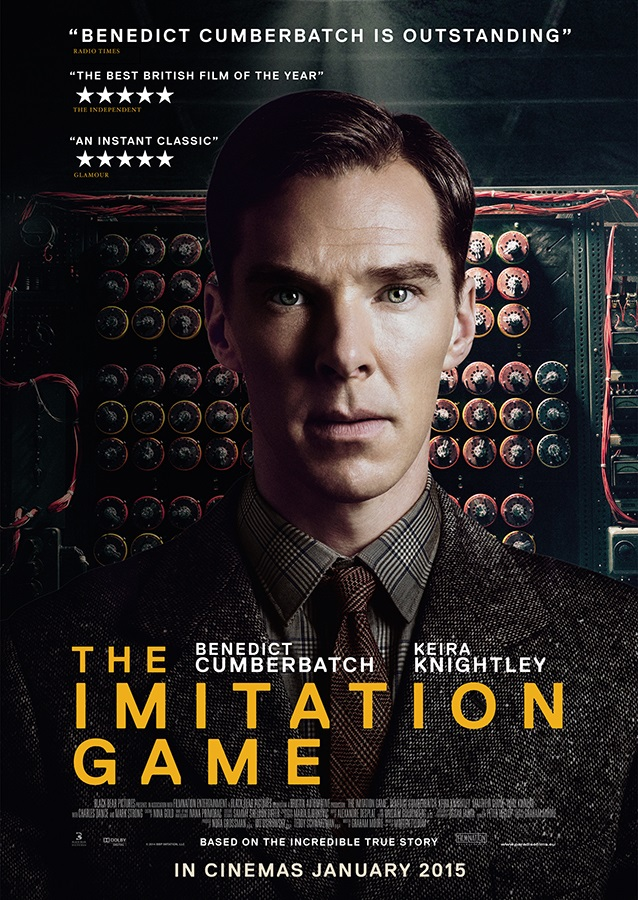
\includegraphics[scale=0.35]{turing/imitationGame}
	\end{frame}
}

%Das hier am Besten hinmalen mit Band und Schreiblesekopf und an der Tafel machen:
\begin{frame}{Eine einfache Turingmaschine}
	\begin{center}
		\begin{tikzpicture}[->,>=stealth,shorten >=1pt,auto,node distance=2.8cm,
		semithick,initial text={}]
		\tikzstyle{every state}=[]
		
		\node[initial,state] (A)                    {$a$};
		\node[state]         (M) [right of=A] 	    {$m$};
		
		\path 
		(A) edge [loop above] node {$\word 1\io\word 0R$} (A)
		edge [loop below]  node {$\word 0\io\word 1R$} (A)
		edge 					  node {$\word{2}\io\word{X}R$} (M)
		(M) edge [loop right] node {$\stackedtight{\word 0\io\word XR \\ \word 1\io\word XR \\ \word 2\io\word XR}$} (M)
		;
		\end{tikzpicture}
	\end{center} \pause
	Macht genau dasselbe wie der Automat ausm letzten Tut. \\ \pause
	\begin{tabular}{rl@{\ \?>\ }rl}
		Zustand vorher: & a &  nachher: & \hphantom{\word{100010}}a \\
		Band vorher: &\word{011101} &  nachher:&  \word{100010}$\9$\\
		\hline
		Zustand vorher: & a &  nachher: & \hphantom{\word{100010}}m \\
		Band vorher: &\word{011102} &  nachher:&  \word{10001X}$\9$\\
		\hline
		Zustand vorher: & a &  nachher: & \hphantom{\word{100010}}m \\
		Band vorher: &\word{012101} &  nachher:&  \word{10XXXX}$\9$\\
	\end{tabular}

\end{frame}



\begin{frame}{Turingmaschinen}
	Eine Turingmaschine besteht aus...
	\begin{itemize}[<+->]
		\item einem unendlichen Band mit einzelnen Zellen, in denen jeweils genau ein Symbol aus dem Bandalphabet steht
		\item einem Schreib-/Lesekopf, der auf genau einer Bandzelle steht
		\item einer Steuerungseinheit (Mealy-Automat), die sich in genau einem Zustand befindet
	\end{itemize}
\end{frame}

\begin{frame}{Funktionsweise der TM}
	In jedem Ausführungsschritt:
	\begin{itemize}[<+->]
		\item TM liest das Symbol, auf dem der Kopf steht
		\item Steuerung entscheidet über die Ausgabe, den Folgezustand und die Bewegung
		\item Ausgabe wird an der aktuellen Position auf das Band geschrieben
		\item Steuerung wechselt in den Folgezustand
		\item Kopf bewegt sich einen Schritt nach links (L) oder rechts (R) oder bleibt stehen (0)
	\end{itemize}
	\pause
	Die TM \textbf{hält}, wenn für einen Zustand und das gelesene Symbol keine Übergänge in der Steuerung definiert sind. \textbf{Eine TM muss nicht halten!} \\
	\impl Es können „Pfeile fehlen“!
\end{frame}

\begin{frame}{Eine einfache Turingmaschine v2}
	\begin{center}
		\begin{tikzpicture}[->,>=stealth,shorten >=1pt,auto,node distance=2.8cm,
		semithick,initial text={}]
		\tikzstyle{every state}=[]
		
		\node[initial,state] (A)                    {$a$};
		
		\path 
		(A) edge [loop above] node {$\word 1\io\word 0R$} (A)
		edge [loop below]  node {$\word 0\io\word 1R$} (A)
		;
		\end{tikzpicture}
	\end{center} \pause
	Pfeil für Eingabe \word 2 fehlt jetzt! \pause \impl TM hört dann einfach auf! \\ \pause
	\begin{tabular}{rl@{\ \?>\ }rl}
		Zustand vorher: & a &  nachher: & \hphantom{\word{100010}}a \\
		Band vorher: &\word{011101} &  nachher:&  \word{100010}$\9$\\
		\hline
		Zustand vorher: & a &  nachher: & \hphantom{\word{10001}}a \\
		Band vorher: &\word{011102} &  nachher:&  \word{100012}\\
		\hline
		Zustand vorher: & a &  nachher: & \hphantom{\word{10}}a \\
		Band vorher: &\word{012101} &  nachher:&  \word{102101}\\
	\end{tabular}
	
\end{frame}

\begin{frame}{Eine einfache Turingmaschine, Rage-Mode!}
	\begin{center}
		\begin{tikzpicture}[->,>=stealth,shorten >=1pt,auto,node distance=2.8cm,
		semithick,initial text={}]
		\tikzstyle{every state}=[]
		
		\node[initial,state] (A)                    {$a$};
		\node[state]         (M) [right of=A] 	    {$m_1$};
		\node[state]         (M2) [right of=M] 	    {$m_2$};
		
		\path 
		(A) edge [loop above] node {$\stackedtight{\word 1\io\word 0R \\ \word 0\io\word 1R}$} (A)
		edge 					  node {$\word{2}\io\word{2}R$} (M)
		(M) edge [loop above] node {$\stackedtight{\word 0\io\word 0R \\ \word 1\io\word 1R \\ \word 2\io\word 2R}$} (M)
		edge 					  node {$\9\io\9L$} (M2)
		(M2) edge [loop right] node {$\stackedtight{\word 0\io\9L \\ \word 1\io\9L \\ \word 2\io\9L}$} (M2)
		;
		\end{tikzpicture}
	\end{center} \pause
	\impl Löscht das komplette Eingabewort, wenn sie ne \word 2 in die Finger kriegt! \smiley \\ \pause
	\begin{tabular}{rl@{\ \?>\ }rl}
		Zustand vorher: & a &  nachher: & \hphantom{\word{100010}}a \\
		Band vorher: &\word{011101} &  nachher:&  \word{100010}$\9$\\
		\hline
		Zustand vorher: & a &  nachher: & $m_2$\\
		Band vorher: &\word{011102} &  nachher:&  $\9\9\9\9\9\9$\\
		\hline
		Zustand vorher: & a &  nachher: & $m_2$ \\
		Band vorher: &\word{012101} &  nachher:& $\9\9\9\9\9\9$\\
	\end{tabular}
\end{frame}

\begin{frame}{Ein-/Ausgabe}
	\begin{block}{Eingabe}
		Am Anfang steht das Eingabewort umgeben von Blanksymbolen auf dem Band, der Kopf steht auf dem ersten Zeichen des Eingabeworts.
	\end{block}
	\pause
	
	\begin{block}{Ausgabe}
		Zwei Möglichkeiten:
		\begin{itemize}[<+->]
			\item Berechnung von Funktionen: Ausgabewort steht am Ende auf dem Band \\
			\impl „normale“ TMen
			\item Erkennen von Sprachen: Halten in akzeptierendem Zustand (Doppelkringel)\\
			\impl Turingmaschinen-\textbf{Akzeptor} \\
				  Wir bezeichnen dann wieder mit $L(T)$ die akzeptierte Sprache \\
				  (Was aufm Band steht, ist dann bloß Nebenrechnung.)
		\end{itemize}
	\end{block}
\end{frame}

\begin{frame}{Konfigurationen}
	Den „Gesamtzustand“ einer Turingmaschine (also akt. Zustand, Bandinhalt und Schreibkopf-Position) nennen wir \textbf{Konfiguration}. \\ \pause
	\medskip
	In GBI schreiben wir dafür das aktuelle Wort auf dem Band und über das Zeichen, auf dem der Kopf grade steht, den Zustand. \\
	Beispiel: \\
	\bigskip
	\mbox{}\hphantom{\word{100}$\9$.\!}z \\
	\mbox{\word{100}$\9$\word{101}}
	
	\pause \bigskip
	(Formalkram dazu: \impl VL!)
\end{frame}

\mycomment{ %TODO Fix. Oder gleich ander Tafel machen.
	\begin{frame}{Beispiel}
		\vspace{-30pt}
		\begin{center}
			
			\begin{tikzpicture}[shorten >=1pt,initial text=,node distance=2cm,auto,->,>=stealth,baseline=(B.base)]
			% \node[state,initial]  (S)                       {$S$};
			\node[state,initial]  (A)          {$A$};
			% \node (nix) [right of=A] {};
			\node[state]          (B) [above right of=A] {$B$};
			\node[state]          (C) [right of=B] {$C$};
			\node[state]          (E) [below right of=A] {$E$};
			\node[state]          (D) [right of=E] {$D$};
			\path[->]
			% (S) edge              node  {$\9\io\9R$} (A)
			(A) edge              node  {$\word 1\io\word XR$} (B)
			(B) edge [loop above] node  {$\word 1\io\word 1R$} ()
			edge              node  {$\9\io\9R$} (C)
			(C) edge [loop above] node  {$\word 1\io\word 1R$} ()
			edge              node  {$\9\io\word 1L$} (D)
			(D) edge [loop below] node  {$\word 1\io\word 1L$} ()
			edge              node  {$\9\io\9L$} (E)
			(E) edge [loop below] node  {$\word 1\io\word 1L$} ()
			edge              node  {$\word X\io\word 1R$} (A)
			% (B) edge              node        {$\9\io\9R$} (B)
			% edge [loop right] node        {$\#1\io\#1R$} ()
			% (B) edge [loop right] node {$\9\io\#1L$} ()
			% edge  node [pos=0.3]       {$\#1\io\#1L$} (A)
			;
			\end{tikzpicture}
			\bigskip
			
			\begin{tabular}{c|c|c|c|c|c}
				%	& A & B & C & D & E \\ \hline
				%	$\square $ & & C,$\square$,R & D, $\word 1$, L & E,$\square$, L & \\ \hline
				%	$\word 1$ & B,$X$, R & B,$\word 1$, R & C,$1$, R & D,$\word 1$, L & E,$\word 1$, L \\ \hline
				%	$X$ & & & & & A,$\word 1$,R \\
			\end{tabular}
		\end{center}
	\end{frame}
	
	% DIESES BEISPIEL IST FEHLERHAFT!
	\begin{frame}[t]{Beispiel}
		\only<1|handout:1>{Eingabe: $11$}
		\bigskip
		\begin{itemize}
			\only<1-3|handout:1>{\item[1] \begin{Messtabelle}{ccccccc} & A & & & & & \\ & $\downarrow$ &&&&& \\ 
					$\square$ & 1 & 1 & $\square$ & $\square$ & $\square$ & $\square$ \end{Messtabelle} }
			\only<2-4|handout:1>{\item[2] \begin{Messtabelle}{ccccccc} &  & B & & & & \\ & &$\downarrow$ &&&& \\ 
					$\square$ & X & 1 & $\square$ & $\square$ & $\square$ & $\square$ \end{Messtabelle} }
			\only<3-5|handout:1>{\item[3] \begin{Messtabelle}{ccccccc} &  & & & C& &  \\ &  &&& $\downarrow$ & &\\ 
					$\square$ & X & 1 & $\square$ & $\square$ & $\square$ & $\square$ \end{Messtabelle} }
			\only<4-6|handout:2>{\item[4] \begin{Messtabelle}{ccccccc} &  & & D & & &  \\ &  && $\downarrow$ &&& \\ 
					$\square$ & X & 1 & $\square$ & 1 & $\square$  & $\square$ \end{Messtabelle} }
			\only<5-7|handout:2>{\item[5]  \begin{Messtabelle}{ccccccc} &  & E &  & & &  \\ &  & $\downarrow$ &&&& \\ 
					$\square$ & X & 1 & $\square$ & 1 & $\square$  & $\square$ \end{Messtabelle} }
			\only<6-8|handout:2>{ \item[6] \begin{Messtabelle}{ccccccc} &  &   A && & &  \\ &  &  $\downarrow$ &&&& \\ 
					$\square$ & 1 & 1 & $\square$ & 1 & $\square$  & $\square$ \end{Messtabelle} }
			\only<7-9|handout:3>{\item[7] \begin{Messtabelle}{ccccccc} &  &    & B & & &  \\ &  &&  $\downarrow$ &&& \\ 
					$\square$ & 1 & X & $\square$ & 1 & $\square$  & $\square$ \end{Messtabelle} }
			\only<8-10|handout:3>{\item[8] \begin{Messtabelle}{ccccccc} &  &    &  & & C &  \\ &  && && $\downarrow$ & \\ 
					$\square$ & 1 & X & $\square$ & 1 & $\square$  & $\square$ \end{Messtabelle} }
			\only<9-11|handout:3>{\item[9] \begin{Messtabelle}{ccccccc} &  &    &  &  D& &  \\ &  && & $\downarrow$ && \\ 
					$\square$ & 1 & X & $\square$ & 1 & 1  & $\square$ \end{Messtabelle} }
			\only<10-12|handout:4>{\item[10] \begin{Messtabelle}{ccccccc} &  &   E &  &  & &  \\ &   & $\downarrow$ && &&\\ 
					$\square$ & 1 & X & $\square$ & 1 & 1  & $\square$ \end{Messtabelle} }
			\only<11-12|handout:4>{\item[11] \begin{Messtabelle}{ccccccc} &  &    & A &  & &  \\ &   && $\downarrow$ && &\\ 
					$\square$ & 1 & 1 & $\square$ & 1 & 1  & $\square$ \end{Messtabelle} }
		\end{itemize}
		\only<12|handout:4>{ Also allgemein : Eingabe von $1^k$ wird zu $\square \, 1^k \, \square \, 1^k \, \square $} 
	\end{frame}
}


\begin{frame}{Turingmaschine}
	\begin{Definition}
		Eine Turingmaschine $T$ ist definiert als $$ T = (Z, z_0 , X, f,g, m)$$
		\begin{itemize}[<+->]
			\item $Z \quad$ Zustandsmenge 
			\item $z_0\in Z \quad$ Startzustand
			\item $X \quad$ Bandalphabet mit $\square \in X$
			\item $f:Z\times X \dashrightarrow Z \quad$ Übergangsfunktion
			\item $g:Z\times X\dashrightarrow X \quad$ Ausgabefunktion  \quad (\textbf{genau ein Zeichen} als Ausgabe!)
			\item $m:Z\times X \dashrightarrow \{\text{L},\text{0},\text{R}\} \quad$ Bewegungsfunktion
		\end{itemize}
		\pause
		Alle Funktionen können auch nur partiell definiert ($\dashrightarrow$) sein. \\
		(Heißt: Sie sind nicht linkstotal $=$ Es fehlen Pfeile.)
	\end{Definition}
\end{frame}

\begin{frame}{Beispiel: Formale Definition}
	\begin{center}
		\begin{tikzpicture}[->,>=stealth,shorten >=1pt,auto,node distance=2.8cm,
		semithick,initial text={}]
		\tikzstyle{every state}=[]
		
		\node[initial,state] (A)                    {$a$};
		\node[state]         (M) [right of=A] 	    {$m_1$};
		\node[state]         (M2) [right of=M] 	    {$m_2$};
		
		\path 
		(A) edge [loop above] node {$\stackedtight{\word 1\io\word 0R \\ \word 0\io\word 1R}$} (A)
		edge 					  node {$\word{2}\io\word{2}R$} (M)
		(M) edge [loop above] node {$\stackedtight{\word 0\io\word 0R \\ \word 1\io\word 1R \\ \word 2\io\word 2R}$} (M)
		edge 					  node {$\9\io\9L$} (M2)
		(M2) edge [loop right] node {$\stackedtight{\word 0\io\9L \\ \word 1\io\9L \\ \word 2\io\9L}$} (M2)
		;
		\end{tikzpicture}
	\end{center}
	\begin{align*}
		\text{Bandalphabet } X &= \set{\word 0, \word 1, \word 2, \9} \\
		f(a,\word 1) &= a	\\
		f(a, \9) &\text{ ist nicht definiert.} \\ 
		g(a, \word 1) &= \word 0 \\
		g(a, \9) &\text{ ist nicht definiert.} \\ 
		m(m_1, \9) &= L \\
		m(m_2, \9) & \text{ ist nicht definiert.}
	\end{align*}
\end{frame}

\begin{frame}{Aufgabe}
	Was macht die folgende Turingmaschine für Eingaben aus $\{\word 0, \word 1\}^*$?
	
	%\smallskip
	%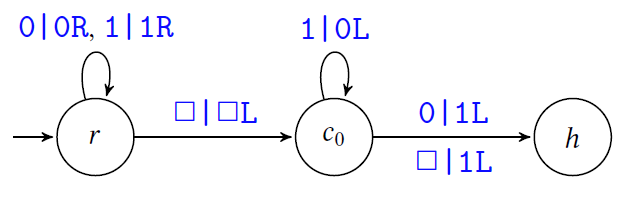
\includegraphics[scale=0.65]{turing/addBin1}
	\begin{center}
		\begin{tikzpicture}[->,>=stealth,shorten >=1pt,auto,node distance=2.8cm,
		semithick,initial text={}]
		\tikzstyle{every state}=[]
		
		\node[initial,state] (R)                    {$r$};
		\node[state]         (C) [right of=R] 	    {$c_0$};
		\node[state]         (H) [right of=C] 	    {$h$};
		
		\path 
		(R) edge [loop above] node {$\word 0\io\word 0R, \word 1\io\word1R$} (R)
		edge 					  node {$\9\io\9L$} (C)
		(C) edge [loop above] node {$\word 1\io\word 0L$} (C)
		edge 					  node {$\stackedtight{\word 0\io\word 1L \\ \9\io\word 1L }$} (H)
		;
		\end{tikzpicture}
	\end{center}
	
	\smallskip
	\visible<2|handout:2>{
		Inkrementieren der dargestellten Zahl um $1$.
	}
\end{frame}

\begin{frame}{Aufgabe}
	Entwerft eine Turingmaschine, die für eine Eingabe $w \in \{\word 0, \word 1\}^*$ $$\fRepr_2(\fNum_2(w) - 1)$$ berechnet. Ihr dürft davon ausgehen, dass $\fNum_2(w) > 0$ gilt.\\
	\visible<2-|handout:2->{
		\begin{center}
			\begin{tikzpicture}[->,>=stealth,shorten >=1pt,auto,node distance=2.8cm,
			semithick,initial text={}]
			\tikzstyle{every state}=[]
			
			\node[initial,state] (R)                    {$r$};
			\node[state]         (C) [right of=R] 	    {$c_0$};
			\node[state]         (H) [right of=C] 	    {$h$};
			
			\visible<4-|handout:3->{
				\node[state]         (Z) [below=1cm of H] 	    {$z$};
			}
			\visible<6-|handout:4->{
				\node[state]         (L) [below=1cm of C] 	    {$\ell$};
			}
			
			\path 
			(R) edge [loop above] node {$\word 0\io\word 0R, \word 1\io\word1R$} (R)
			edge 					  node {$\9\io\9L$} (C)
			(C) edge [loop above] node {$\word 0\io\word 1L$} (C)
			edge 					  node {$\word 1\io\word 0L$} (H);
			
			\visible<4-|handout:3->{
				\path
				(H) edge [loop above] node {$\word 0\io\word 0L, \word 1\io\word1L$} (H)
				edge [left]				  node {$\9\io\9R$} (Z)
				(Z)  edge [loop right] node {$\word 0\io\9R$} (Z);
			}
			
			\visible<6-|handout:4->{
				\path
				(Z)  edge 				 node[below] {$\9\io\word 0L$} (L);
			}
			\end{tikzpicture}
		\end{center}
	}
	\visible<3-|handout:3->{\§{\textbf{Achtung}:} Was passiert mit führenden Nullen?} \\ 
	\visible<5-|handout:4->{\. Was, wenn es nur eine \word 0 gibt?} \\	
\end{frame}

\begin{frame}{Aufgabe}
	Wie würde man eine (einfache, nicht effiziente) TM zum Addieren von zwei Zahlen in Binärdarstellung aufbauen? \\ \pause
	\smallskip
	\impl Inkrementiere erste Zahl, dekrementiere zweite Zahl. Wiederhole, bis zweite Zahl $= 0$.
\end{frame}

\def\bword#1{\texttt{#1}}
\begin{frame}[t]{TM-Akzeptoren}
	\only<all:1>{
		Erinnerung: Inkrementieren um eins 
		\begin{center}
			\begin{tikzpicture}[->,>=stealth,shorten >=1pt,auto,node distance=2.8cm,
				semithick,initial text={}]
				\tikzstyle{every state}=[]
				
				\node[initial,state] (R)                    {$r$};
				\node[state]         (C) [right of=R] 	    {$c_0$};
				\node[state]         (H) [right of=C] 	    {$h$};
				
				\node[state,accepting,white]         (A) [below of=H] 	    {\phantom{$a_1$}};
				\node[state,white]         (B) [below of=C] 	    {\phantom{$a_2$}};
				
				\path 
				(R) edge [loop above] node {$\word 0\io\word 0R, \word 1\io\word 1R$} (R)
				edge 					  node {$\9\io\9L$} (C)
				(C) edge [loop above] node {$\word 1\io\word 0L$} (C)
				edge 					  node {$\stackedtight{\word 0\io\word 1L \\ \9\io\word 1L}$} (H)
				
				(H) edge [loop above,white] node {\phantom{$\word 0\io\word 0L, \word 1\io\word 1L$}} (H)
				(A)  edge [white]				 node[below] {\phantom{$\word 0\io\word 0L$}} (B)
				;
			\end{tikzpicture}
		\end{center}
	\mbox{}\vphantom{Welche Sprache....} \\
	}
	\only<all:2->{
		\?> TM-Akzeptor: 
		\begin{center}
			\begin{tikzpicture}[->,>=stealth,shorten >=1pt,auto,node distance=2.8cm,
				semithick,initial text={},every initial by arrow/.style={gray}]
				\tikzstyle{every state}=[]
				
				\node[initial,state,gray] (R)                    {$r$};
				\node[state,gray]         (C) [right of=R] 	    {$c_0$};
				\node[state]         (H) [right of=C] 	    {$h$};
				
				\node[state,accepting]         (A) [below of=H] 	    {$a_1$};
				\node[state]         (B) [below of=C] 	    {$a_2$};
				
				\path 
				(R) edge [loop above,gray] node {$\bword 0\io\bword 0R, \bword 1\io\bword 1R$} (R)
				edge [gray] 					  node {$\9\io\9L$} (C)
				(C) edge [loop above,gray] node {$\bword 1\io\bword 0L$} (C)
				edge [gray] 					  node {$\stackedtight{\bword 0\io\bword 1L \\ \9\io\bword 1L}$} (H)
				
				(H) edge [loop above] node {$\word 0\io\word 0L, \word 1\io\word 1L$} (H)
				edge [left]				  node {$\9\io\9R$} (A)
				(A)  edge [loop above left] node[left] {$\word 1\io\word 1R$} (A)
				(A)  edge 				 node[below] {$\word 0\io\word 0R$} (B)
				;
			\end{tikzpicture}
		\end{center}
		Welche Sprache akzeptiert diese TM? \\
	}
	\medskip
	\visible<3->{$\impl L(T) = \set{w \in \set{\word 0,\word 1}^* \Mid \fRepr_2(\fNum_2(w) + 1) \in \set{\word 1}^*}$}
\end{frame}

\begin{frame}{Turing-Maschinen vs. Supercomputer}
	Eine TM kann \textbf{genauso viel} berechnen wie euer Handy oder ein Supercomputer von Intel. {\small (Bloß halt etwas langsamer und umständlicher!)} \\
	\medskip
	Es gibt kein „mächtigeres“ Maschinenmodell als Turingmaschinen. \\
	\only<beamer:0>{
		\medskip 
		\begin{center}
			\impl Was eine Turingmaschine nicht berechnen \\ kann, kann keiner berechnen. \smiley \\ \#Prädikatenlogik-Blatt 2017/18
		\end{center}
	}
\end{frame}

\mycomment{ % Formalkram ist bähhh...
	% Ja, aber eigentlich wichtig. Aber dieses Jahr keine Zeit.
	\begin{frame}{Konfiguration}
		\begin{Definition}
			Als \textbf{Konfiguration} $ c =(z,b,p)$ bezeichnen wir den Zustand einer Turing-Maschine zu einem Zeitpunkt. Dabei ist 
			\begin{itemize}
				\item $z\in Z$ der Zustand
				\item $b: \Z\to X$ die Bandbeschriftung
				\item $p\in \Z$ die Position des Zeigers.
			\end{itemize}
		\end{Definition}
	\end{frame}
	
	\begin{frame}{Berechnungsschritte}
		\begin{Definition}
			In einem Berechnungsschritt geht eine TM aus einer Konfiguration $c$ 
			in die Konfiguration $$\Delta_1(c) := c' = (z',b',p')$$ über, wobei gilt:
			\begin{itemize}[<+->]
				\item $z' = f(z,b(p))$
				\item $\forall i\in \Z: b'(i) =
				\begin{cases}
				b(i) & \text{ falls } i\not=p \\
				g(z,b(p)) & \text{ falls } i=p
				\end{cases}$
				\item $p' = p + m(z,b(p))$
			\end{itemize}
			\bigskip
			
			\pause
			Wenn $\Delta_1(c)$ nicht definiert ist, bezeichnet man $c$ als \textbf{Endkonfiguration} und die TM \textbf{hält}.
		\end{Definition}
	\end{frame}
	
	\begin{frame}{Berechnungen}
		\begin{Definition}
			Eine Berechnung ist eine Folge von Konfigurationen $(c_0, c_1, ..., c_t)$ bei der gilt $$c_{i+1} = \Delta_1(c_i)$$ \pause
			Es gibt endliche, haltende (endet in einer Endkonfiguration) und unendliche Berechnungen.
			\bigskip
			
			\pause
			Induktiv definiert man $\Delta_t(c) , t\in\N_0$ als die Konfiguration, welche nach $t$ Berechnungsschritten erreicht werden kann und $\Delta_*(c)$ als Endkonfiguration, die von $c$ aus erreicht wird (falls die Berechnung endet).
		\end{Definition}
	\end{frame}
}








\begin{frame}{Entscheidbarkeit}
	\begin{Definition}
		Eine Sprache $L$ ist eine   
		\begin{itemize}[<+->]
			\item \textbf{aufzählbare Sprache}, wenn es eine Turingmaschine gibt, die $L$ akzeptiert.
			\item \textbf{entscheidbare Sprache}, wenn es eine Turingmaschine gibt, die $L$ akzeptiert und \emph{für jede Eingabe} hält.
		\end{itemize}
	\end{Definition} \pause
	
	Bei aufzählbaren Sprachen ist nicht definiert, wie sich die TM für Wörter $ w \notin L$ verhält. Sie kann diese ablehnen oder nicht halten. Ob eine TM für eine Eingabe nicht hält, können wir \enquote{von außen} nicht einfach feststellen.
\end{frame}


\begin{frame}{Aufgabe}
	Entwerft eine Turingmaschine, die die Sprache $ \{\word 0^k\word 1^k \mid k\in \N_0 \} $ akzeptiert.
	% TODO Lösung
\end{frame}

\begin{frame}{Aufgabe}
	Entwerft eine TM, die alle gültigen Klammerausdrücke entscheidet.\\
	\medskip
	Gültige Klammerausdrücke werden dabei von der folgenden Grammatik produziert: $ G = (\{S\},\{\word (, \word )\}, S, P )$ mit den Produktionen $\set{ S \to \eps \mid \word (S\word )S}$.
	% TODO Lösung
\end{frame}


\section{Komplexität}
\begin{frame}[plain] \large \bf \centering
	Wir betrachten zuerst nur Turingmaschinen, die bei jedem Eingabewort halten!
\end{frame}

\subsection{Berechnungskomplexität}
\begin{frame}{Zeitkomplexität}
	\begin{Definition}
		Die Zeitkomplexität Time$(n)$ einer Turingmaschine ist die maximale Anzahl an Schritten, die eine Turingmaschine bei Eingabe eines Worts der Länge $n$ benötigen kann (worst-case).
	\end{Definition}
	\pause
	\textbf{Beispiel:} Überprüfung auf Palindrom:
	\begin{itemize}[<+->]
		\item Erstes Symbol -> letztes Symbol ($n$) 
		\item Zurück zum ersten ($n$)
		\item Mit kürzerem Wort wiederholen ($|n-2|$)
	\end{itemize} \pause
	Also insgesamt $$T(n) \leq 2n + 1 + T(n-2)$$ 
	Daraus folgern wir $$T(n) \in O(n^2)$$
\end{frame}

\begin{frame}{Platzkomplexität}
	\begin{Definition}
		Die Platzkomplexität Space$(n)$ einer Turingmaschine ist die maximale Anzahl an Feldern, die eine Turingmaschine bei Eingabe eines Worts der Länge $n$ benötigen kann (worst-case). Benötigt wird ein Feld, wenn es vom Schreibkopf besucht wird oder von der Eingabe belegt wurde.
	\end{Definition}
	\pause
	\textbf{Beispiel:} Überprüfung auf Palindrom:
	\begin{itemize}[<+->]
		\item Erstes Symbol -> letztes Symbol ($n + 1$) 
		\item Zurück zum ersten ($0$)
		\item Mit kürzerem Wort wiederholen ($0$)
	\end{itemize} \pause
	Also insgesamt $$n+1 \in \Th{n}$$
\end{frame}

\begin{frame}{Platzkomplexität}
	Wie hängen Zeit- und Platzkomplexität zusammen?
	\begin{itemize}
		\item Wenn eine TM nur $n$ Schritte macht, kann sie auch nur $n$ Felder besuchen
		\item Aber anders herum: Auch mit $n$ Feldern können exponentiell viele Schritte durchgeführt werden.\\
			  Beispiel: Band mit $0^n$. Solange inkrementieren (siehe Aufgabe), bis $1^n$ auf dem Band steht. \pause Also $2^n - 1$ mal inkrementieren, somit mindestens $2^n - 1$ Schritte.
	\end{itemize}
\end{frame}

\begin{frame}
	\begin{Definition}
	\begin{itemize}
		\item \textbf{P} ist die Menge aller Entscheidungsprobleme, die von Turingmaschinen entschieden werden können, deren Zeitkomplexität polynomiell ist.
		\item \textbf{PSPACE} ist die Menge aller Entscheidungsprobleme, die von Turingmaschinen entschieden werden können, deren Raumkomplexität polynomiell ist.
	\end{itemize}
	\end{Definition}
	\pause
	Es ist $$\textbf{P} \subset \textbf{PSPACE}$$ \pause
	Die andere Richtung ist \textbf{ein großes offenes Problem}\\
	Wir haben zwar ein Beispiel für eine TM mit polynomiellen Platz und exponentieller Zeit gesehen, aber das \textbf{Problem} (alle $0$ zu $1$ umwandeln) hätte man deutlich effizienter lösen können.
\end{frame}

\subsection{Aufgabe}
\begin{frame}{Aufgabe} %(WS 2011)
	\only<1|handout:1>{	
		Die Turingmaschine $T$ mit Anfangszustand $S$ sei durch folgende Überführungsfunktion gegeben 
		\begin{table}[H]
		\centering
		\begin{tabular}{c|c|c|c|c}
		& $S$ & $S_a$ & $S_b$ & $R$ \\
		\hline
		$a$ & $(X,S_a,L)$ & $(a,S_a,L)$ & $(a,S_b,L)$ & $(a,R,R)$\\
		$b$ & $(X,S_b,L)$ & $(b,S_a,L)$ & $(b,S_b,L)$ & $(b,R,R)$\\
		$X$ & $(X,S,R)$ & $(X,S_a,L)$ & $(X,S_b,L)$ & $(X,S,R)$ \\
		$\square$ & - & $(a,R,R)$ & $(b,R,R)$ & -
		\end{tabular} 
		\end{table}
		\smallskip
		
		Tipp: Manchmal hilft es, die TM zu zeichnen.
	}

	\begin{itemize}
		\item Was steht bei der Eingabe des Wortes $w\in \{a,b\}^*$ am Ende der Berechnung auf dem Band? \\
			\only<2|handout:2>{\emph{Lösung}: Am Ende steht das Wort $R(w)\mathtt X^{\vert w \vert}$ auf dem Band, wobei $R(w)$ das Spiegelbild von $w$ ist.}
		\item Welche Platzkomplexität hat $T$?\\
			\only<2|handout:2>{\emph{Lösung}: Eingabe der Länge $n$: Platzbedarf ist $2n+1$}
		\item Geben Sie eine einfache Funktion $f:\nN_0 \to \nN_0$ an, so dass die Zeitkomplexität von $T$ in $\Theta(f(n))$ liegt.\\
			\only<2|handout:2>{\emph{Lösung}: Eingabe der Länge $n$: Zeitbedarf in $\Theta(n^2)$ \\}
	\end{itemize}
\end{frame}

\subsection{Unentscheidbare Probleme}
\begin{frame}{Unentscheidbare Probleme}
	Es existieren Probleme, die von keiner Turingmaschine entschieden werden können.\\ \pause
	Erinnerung: Entscheidbar heißt, dass es eine Turingmaschine gibt, die für jede Eingabe hält und entscheiden kann, ob das Wort in der Sprache liegt oder nicht. Statt Sprachen spricht man auch gerne von Problemen.\\ \pause
	
	\bigskip
	Achtung: Unentscheidbar meint wirklich \enquote{hält für manche Eingaben nie} und nicht \enquote{braucht $2^{2^{2^{n}}}$ Zeit}.
\end{frame}

\begin{frame}{Codierung von Turingmaschinen}
	In der VL: Codierung einer Turingmaschine als Wort über dem Alphabet \nolinebreak $\{0,1,[,]\} \qquad$ (Gödelisierung)
	\bigskip
	
	\begin{Satz}
		Es existiert eine universelle Turingmaschine $U$, die für zwei Eingaben $[\mathtt w_1][\mathtt w_2]$ 
		\begin{itemize}
			\item überprüft ob $\mathtt w_1$ eine Turingmaschine $T$ codiert
			\item falls ja, die Eingabe $\mathtt w_2$ auf dieser Turingmaschine simuliert
			\item Das Ergebnis davon berechnet (falls $T$ hält)
		\end{itemize}
	\end{Satz}
\end{frame}

\begin{frame}{Halteproblem}
	\begin{Satz}
		Es ist nicht möglich eine Turingmaschine $H$ zu bauen, die für jede Turingmaschine $T$ und jede Eingabe $w$ entscheidet, ob $T$ bei der Eingabe von $w$ hält.
	\end{Satz}
\end{frame}

\begin{frame}{Beweis}
	Sei eine Tabelle $x_i, f_j$ gegeben, wobei die $x_i$ alle Codierungen einer Turingmaschine sind und die $f_j$ die berechneten Funktionen der Turingmaschine $T_j$ sind. Sei jetzt $H$ eine TM, die das Halteproblem löst und $G$ eine Maschine, die \begin{itemize}
		\item Wenn $H$ mitteilt, dass $T_{x_i} ( x_i )$ hält, dann geht $G$ in eine Endlosschleife.
		\item Wenn $H$ mitteilt, dass $T_{x_i} ( x_i )$ nicht hält, dann hält $G$
	\end{itemize}
	Jede mögliche Turingmaschine $T_{x_i}$ verhält sich also für die Eingabe $x_i$ genau anders wie $G$. Also ist $G$ eine Turingmaschine, die nicht in der Tabelle liegt, aber in der Tabelle sind alle TMs enthalten, da diese ja abzählbar sind. Widerspruch!
\end{frame}

\begin{frame}{Beweis 2}
	Sei wieder $H$ eine TM, die das Halteproblem löst und $G$ eine Maschine, die \begin{itemize}
		\item Wenn $H$ mitteilt, dass $T_{x_i} ( x_i )$ hält, dann geht $G$ in eine Endlosschleife.
		\item Wenn $H$ mitteilt, dass $T_{x_i} ( x_i )$ nicht hält, dann hält $G$
	\end{itemize}
	Also gilt: $$ G \text{ hält für Eingabe } w \iff T_w \text{ hält nicht für Eingabe } w $$
	Setzen wir nun für $w$ die Codierung von $G$ ein, so erhalten wir:
	$$ G \text{ hält für Eingabe } w \iff G \text{ hält nicht für Eingabe } w $$
	Widerspruch!
\end{frame}

\begin{frame}{Fleißige Biber}
	\begin{Definition}
		Ein fleißiger Biber ist eine Turingmaschine, die $n+1$ Zustände hat, wobei ein Anfangszustand und ein Haltezustand darunter sind und die nur Einsen produzieren kann.
	\end{Definition}
	\pause

	\begin{Definition}
		Als Busy-Beaver-Funktion $bb(n)$ wird die maximale Anzahl an Einsen bezeichnet, die ein fleißiger Bieber mit $n+1$ Zuständen auf dem Band hinterlassen kann.
	\end{Definition} 

	\begin{Satz}
		Die Busy-Beaver-Funktion ist nicht berechenbar (es gibt keine Turingmaschine, die die Funktionswerte als Ausgabe liefert).
	\end{Satz}
\end{frame}

% TODO: Aufgaben!


\begin{frame}{Turingmaschinen: Klausur}
	Noch ein Hinweis zum Schluss:\\
	Bisher kam in {\tiny fast} \textbf{jeder} Klausur eine Aufgabe zu Turingmaschinen dran.\\
	Diese gibt meist relativ viele Punkte.\\
	
	\bigskip
	Zu 99 \% wird auch dieses Mal wieder eine TM-Aufgabe drankommen.\\
	\textbf{Also übt das!} Hier zählt vor allem Geschwindigkeit (und Präzision).
\end{frame}

\def\abbrsize{\footnotesize}
\begin{frame}	
	\begin{block}{Was ihr nun wissen solltet}
		\begin{itemize}
			\item Turingmaschinen
			\item Komplexität
			\item Entscheidbarkeit -- Wir können alles. Außer Halteproblem. Und so Zeug.
		\end{itemize}
	\end{block}
	
	\begin{block}{Und so geht es weiter...}
		\vspace{-.3\baselineskip}
		\begin{itemize}
			\item Algorithmen I -- Mehr zu Algorithmen, Laufzeiten, Datenstrukturen, Graphen
			\item \textbf{T}{\abbrsize echnische} \textbf{I}{\abbrsize nformatik} -- Realisierung von Schaltungen, Prozessoren (MIMA, ...)
			\item \textbf{T}{\abbrsize heoretische} \textbf{G}{\abbrsize rundlagen der} \textbf{I}{\abbrsize nformatik} -- Mehr zu Grammatiken, Komplexität, Entscheidbarkeit, Turingmaschinen
		\end{itemize}
	\end{block}
\end{frame}

\thassedaniel{
	\begin{frame}{Falls ihr mehr wollt...}
		\begin{block}{Persönliche Empfehlungen}
			\begin{itemize}
				\item Design and Analysis of Algorithms (für Algorithmen I)
				\item CS50x
				\item From Nand to Tetris
				\item ICPC-Basispraktikum
			\end{itemize}
		\end{block}
		
		\begin{itemize}
			\item EDX (edx.org)
			\item Coursera (coursera.org)
		\end{itemize}
	\end{frame}
}{
\begin{frame}{Falls ihr mehr wollt...} % S. o.
	\begin{block}{Persönliche Empfehlungen}
		\begin{itemize}
			\item ICPC-Basispraktikum
		\end{itemize}
	\end{block}
\end{frame}
}


\begin{frame}{Das war GBI}
	\begin{columns}
		\pause
		\column{0.4\linewidth}
		\begin{figure}[H]
			\vspace{-20pt}
			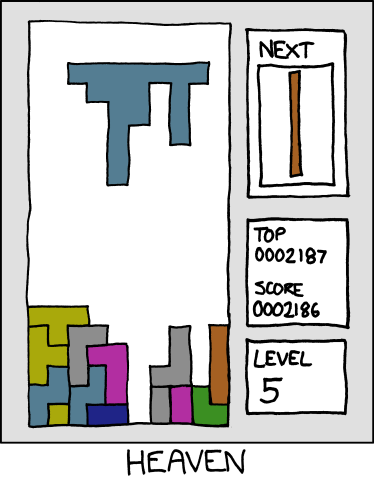
\includegraphics[scale=0.45]{xkcd/heaven}
		\end{figure}
	
		\pause
		\column{0.5\linewidth}
		\begin{figure}[H]
			\vspace{-20pt}
			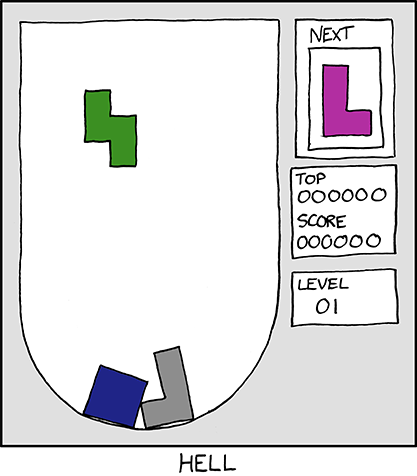
\includegraphics[scale=0.45]{xkcd/hell}
		\end{figure}
	\end{columns}
\end{frame}

\begin{headframe}[ Viel Erfolg  bei \\ euren Klausuren! \smiley]
	--- The End ---
\end{headframe}

% Scheint leider kein vernünftiges Abschieds-XKCD zu geben
\thasse{
	\xkcdframe{5.8}{30}{xkcd/np_complete.png}{http://www.xkcd.com}{}
}

\slideThanks

\end{document}